% Options for packages loaded elsewhere
% Options for packages loaded elsewhere
\PassOptionsToPackage{unicode}{hyperref}
\PassOptionsToPackage{hyphens}{url}
\PassOptionsToPackage{dvipsnames,svgnames,x11names}{xcolor}
%
\documentclass[
  letterpaper,
  DIV=11,
  numbers=noendperiod]{scrartcl}
\usepackage{xcolor}
\usepackage{amsmath,amssymb}
\setcounter{secnumdepth}{-\maxdimen} % remove section numbering
\usepackage{iftex}
\ifPDFTeX
  \usepackage[T1]{fontenc}
  \usepackage[utf8]{inputenc}
  \usepackage{textcomp} % provide euro and other symbols
\else % if luatex or xetex
  \usepackage{unicode-math} % this also loads fontspec
  \defaultfontfeatures{Scale=MatchLowercase}
  \defaultfontfeatures[\rmfamily]{Ligatures=TeX,Scale=1}
\fi
\usepackage{lmodern}
\ifPDFTeX\else
  % xetex/luatex font selection
\fi
% Use upquote if available, for straight quotes in verbatim environments
\IfFileExists{upquote.sty}{\usepackage{upquote}}{}
\IfFileExists{microtype.sty}{% use microtype if available
  \usepackage[]{microtype}
  \UseMicrotypeSet[protrusion]{basicmath} % disable protrusion for tt fonts
}{}
\makeatletter
\@ifundefined{KOMAClassName}{% if non-KOMA class
  \IfFileExists{parskip.sty}{%
    \usepackage{parskip}
  }{% else
    \setlength{\parindent}{0pt}
    \setlength{\parskip}{6pt plus 2pt minus 1pt}}
}{% if KOMA class
  \KOMAoptions{parskip=half}}
\makeatother
% Make \paragraph and \subparagraph free-standing
\makeatletter
\ifx\paragraph\undefined\else
  \let\oldparagraph\paragraph
  \renewcommand{\paragraph}{
    \@ifstar
      \xxxParagraphStar
      \xxxParagraphNoStar
  }
  \newcommand{\xxxParagraphStar}[1]{\oldparagraph*{#1}\mbox{}}
  \newcommand{\xxxParagraphNoStar}[1]{\oldparagraph{#1}\mbox{}}
\fi
\ifx\subparagraph\undefined\else
  \let\oldsubparagraph\subparagraph
  \renewcommand{\subparagraph}{
    \@ifstar
      \xxxSubParagraphStar
      \xxxSubParagraphNoStar
  }
  \newcommand{\xxxSubParagraphStar}[1]{\oldsubparagraph*{#1}\mbox{}}
  \newcommand{\xxxSubParagraphNoStar}[1]{\oldsubparagraph{#1}\mbox{}}
\fi
\makeatother


\usepackage{longtable,booktabs,array}
\newcounter{none} % for unnumbered tables
\usepackage{calc} % for calculating minipage widths
% Correct order of tables after \paragraph or \subparagraph
\usepackage{etoolbox}
\makeatletter
\patchcmd\longtable{\par}{\if@noskipsec\mbox{}\fi\par}{}{}
\makeatother
% Allow footnotes in longtable head/foot
\IfFileExists{footnotehyper.sty}{\usepackage{footnotehyper}}{\usepackage{footnote}}
\makesavenoteenv{longtable}
\usepackage{graphicx}
\makeatletter
\newsavebox\pandoc@box
\newcommand*\pandocbounded[1]{% scales image to fit in text height/width
  \sbox\pandoc@box{#1}%
  \Gscale@div\@tempa{\textheight}{\dimexpr\ht\pandoc@box+\dp\pandoc@box\relax}%
  \Gscale@div\@tempb{\linewidth}{\wd\pandoc@box}%
  \ifdim\@tempb\p@<\@tempa\p@\let\@tempa\@tempb\fi% select the smaller of both
  \ifdim\@tempa\p@<\p@\scalebox{\@tempa}{\usebox\pandoc@box}%
  \else\usebox{\pandoc@box}%
  \fi%
}
% Set default figure placement to htbp
\def\fps@figure{htbp}
\makeatother





\setlength{\emergencystretch}{3em} % prevent overfull lines

\providecommand{\tightlist}{%
  \setlength{\itemsep}{0pt}\setlength{\parskip}{0pt}}



 


\KOMAoption{captions}{tableheading}
\makeatletter
\@ifpackageloaded{caption}{}{\usepackage{caption}}
\AtBeginDocument{%
\ifdefined\contentsname
  \renewcommand*\contentsname{Table of contents}
\else
  \newcommand\contentsname{Table of contents}
\fi
\ifdefined\listfigurename
  \renewcommand*\listfigurename{List of Figures}
\else
  \newcommand\listfigurename{List of Figures}
\fi
\ifdefined\listtablename
  \renewcommand*\listtablename{List of Tables}
\else
  \newcommand\listtablename{List of Tables}
\fi
\ifdefined\figurename
  \renewcommand*\figurename{Figure}
\else
  \newcommand\figurename{Figure}
\fi
\ifdefined\tablename
  \renewcommand*\tablename{Table}
\else
  \newcommand\tablename{Table}
\fi
}
\@ifpackageloaded{float}{}{\usepackage{float}}
\floatstyle{ruled}
\@ifundefined{c@chapter}{\newfloat{codelisting}{h}{lop}}{\newfloat{codelisting}{h}{lop}[chapter]}
\floatname{codelisting}{Listing}
\newcommand*\listoflistings{\listof{codelisting}{List of Listings}}
\makeatother
\makeatletter
\makeatother
\makeatletter
\@ifpackageloaded{caption}{}{\usepackage{caption}}
\@ifpackageloaded{subcaption}{}{\usepackage{subcaption}}
\makeatother
\usepackage{bookmark}
\IfFileExists{xurl.sty}{\usepackage{xurl}}{} % add URL line breaks if available
\urlstyle{same}
% fallback for those not using the hyperref driver hyperxmp:
\makeatletter
\@ifundefined{xmpquote}{\newcommand{\xmpquote}[1]{#1}}{}
\makeatother
\hypersetup{
  pdftitle={NeuralBandit Metric Mapping},
  colorlinks=true,
  linkcolor={blue},
  filecolor={Maroon},
  citecolor={Blue},
  urlcolor={Blue},
  pdfcreator={LaTeX via pandoc}}


\title{NeuralBandit Metric Mapping}
\author{}
\date{}
\begin{document}
\maketitle


\begin{longtable}[]{@{}lrrr@{}}
\caption{Runs found per condition (check: same number of seeds and steps
everywhere).}\tabularnewline
\toprule\noalign{}
condition & seeds & min\_steps & max\_steps \\
\midrule\noalign{}
\endfirsthead
\toprule\noalign{}
condition & seeds & min\_steps & max\_steps \\
\midrule\noalign{}
\endhead
\bottomrule\noalign{}
\endlastfoot
gamma = 0.01 & 5 & 1e+05 & 1e+05 \\
gamma = 0.05 & 5 & 1e+05 & 1e+05 \\
gamma = 0.10 & 5 & 1e+05 & 1e+05 \\
gamma\_model = 0.01 & 5 & 1e+05 & 1e+05 \\
gamma\_model = 0.05 & 5 & 1e+05 & 1e+05 \\
gamma\_model = 0.20 & 5 & 1e+05 & 1e+05 \\
gamma\_model = 0.30 & 5 & 1e+05 & 1e+05 \\
Leaky ReLU + gamma\_model = 0.30 & 5 & 1e+05 & 1e+05 \\
Leaky ReLU & 5 & 1e+05 & 1e+05 \\
ReLU & 5 & 1e+05 & 1e+05 \\
Sigmoid (default) & 5 & 1e+05 & 1e+05 \\
Tanh & 5 & 1e+05 & 1e+05 \\
Tanh + gamma\_model = 0.30 & 5 & 1e+05 & 1e+05 \\
\end{longtable}

\section{Summary across seeds}\label{summary-across-seeds}

Mean and 95\% confidence half-width (t distribution) over seeds.
Recovery rate is the fraction of drifts with a detected recovery; a
drift on the final step is excluded.

{\def\LTcaptype{none} % do not increment counter
\begin{longtable}[]{@{}
  >{\raggedright\arraybackslash}p{(\linewidth - 12\tabcolsep) * \real{0.2500}}
  >{\raggedleft\arraybackslash}p{(\linewidth - 12\tabcolsep) * \real{0.0469}}
  >{\raggedright\arraybackslash}p{(\linewidth - 12\tabcolsep) * \real{0.1094}}
  >{\raggedright\arraybackslash}p{(\linewidth - 12\tabcolsep) * \real{0.1484}}
  >{\raggedright\arraybackslash}p{(\linewidth - 12\tabcolsep) * \real{0.1484}}
  >{\raggedright\arraybackslash}p{(\linewidth - 12\tabcolsep) * \real{0.1562}}
  >{\raggedright\arraybackslash}p{(\linewidth - 12\tabcolsep) * \real{0.1406}}@{}}
\toprule\noalign{}
\begin{minipage}[b]{\linewidth}\raggedright
Condition
\end{minipage} & \begin{minipage}[b]{\linewidth}\raggedleft
Seeds
\end{minipage} & \begin{minipage}[b]{\linewidth}\raggedright
Recovery rate
\end{minipage} & \begin{minipage}[b]{\linewidth}\raggedright
Mean recovery time
\end{minipage} & \begin{minipage}[b]{\linewidth}\raggedright
Reward at recovery
\end{minipage} & \begin{minipage}[b]{\linewidth}\raggedright
Mean rolling reward
\end{minipage} & \begin{minipage}[b]{\linewidth}\raggedright
Final cum. regret
\end{minipage} \\
\midrule\noalign{}
\endhead
\bottomrule\noalign{}
\endlastfoot
Sigmoid (default) & 5 & 0.69 ± 0.14 & 2620 ± 257 & 0.231 ± 0.037 & 0.229
± 0.034 & 77126 ± 3259 \\
ReLU & 5 & 0.81 ± 0.10 & 2758 ± 277 & 0.286 ± 0.106 & 0.283 ± 0.090 &
71714 ± 8993 \\
Tanh & 5 & 0.82 ± 0.16 & 2755 ± 187 & 0.329 ± 0.081 & 0.323 ± 0.071 &
67560 ± 7191 \\
Leaky ReLU & 5 & 0.84 ± 0.05 & 2754 ± 213 & 0.339 ± 0.094 & 0.324 ±
0.088 & 67593 ± 8795 \\
gamma = 0.01 & 5 & 0.62 ± 0.07 & 2636 ± 402 & 0.171 ± 0.026 & 0.177 ±
0.015 & 82399 ± 1299 \\
gamma = 0.05 & 5 & 0.65 ± 0.14 & 2616 ± 289 & 0.242 ± 0.050 & 0.249 ±
0.043 & 75134 ± 4221 \\
gamma = 0.10 & 5 & 0.66 ± 0.21 & 2657 ± 128 & 0.249 ± 0.028 & 0.233 ±
0.041 & 76588 ± 4159 \\
gamma\_model = 0.01 & 5 & 0.78 ± 0.05 & 2749 ± 243 & 0.233 ± 0.045 &
0.235 ± 0.050 & 76502 ± 4815 \\
gamma\_model = 0.05 & 5 & 0.65 ± 0.10 & 2617 ± 184 & 0.229 ± 0.046 &
0.232 ± 0.043 & 76834 ± 4175 \\
gamma\_model = 0.20 & 5 & 0.71 ± 0.07 & 2715 ± 186 & 0.230 ± 0.048 &
0.230 ± 0.044 & 77056 ± 4250 \\
gamma\_model = 0.30 & 5 & 0.69 ± 0.19 & 2605 ± 440 & 0.230 ± 0.044 &
0.226 ± 0.042 & 77430 ± 4084 \\
Tanh + gamma\_model = 0.30 & 5 & 0.93 ± 0.07 & 2873 ± 199 & 0.348 ±
0.077 & 0.339 ± 0.068 & 65889 ± 6820 \\
Leaky ReLU + gamma\_model = 0.30 & 5 & 0.87 ± 0.06 & 2740 ± 250 & 0.288
± 0.089 & 0.294 ± 0.082 & 70680 ± 8414 \\
\end{longtable}
}

\section{Rolling reward by
experiment}\label{rolling-reward-by-experiment}

Lines are the mean over seeds; bands are one standard deviation. Dashed
red lines are drifts and the dotted grey line is the random-action level
(1/7).

\pandocbounded{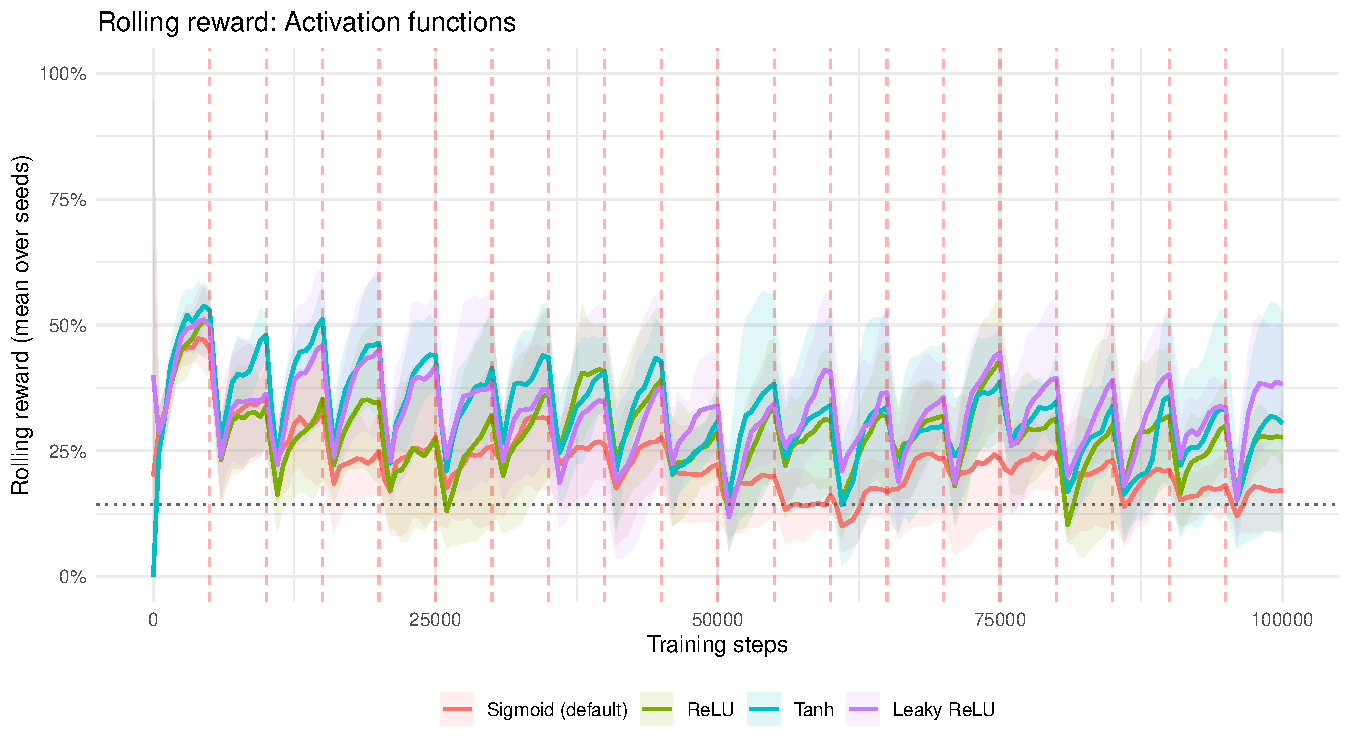
\includegraphics[keepaspectratio]{NeuralBandit_Metric_Mapping_files/figure-pdf/curves-1.pdf}}

\pandocbounded{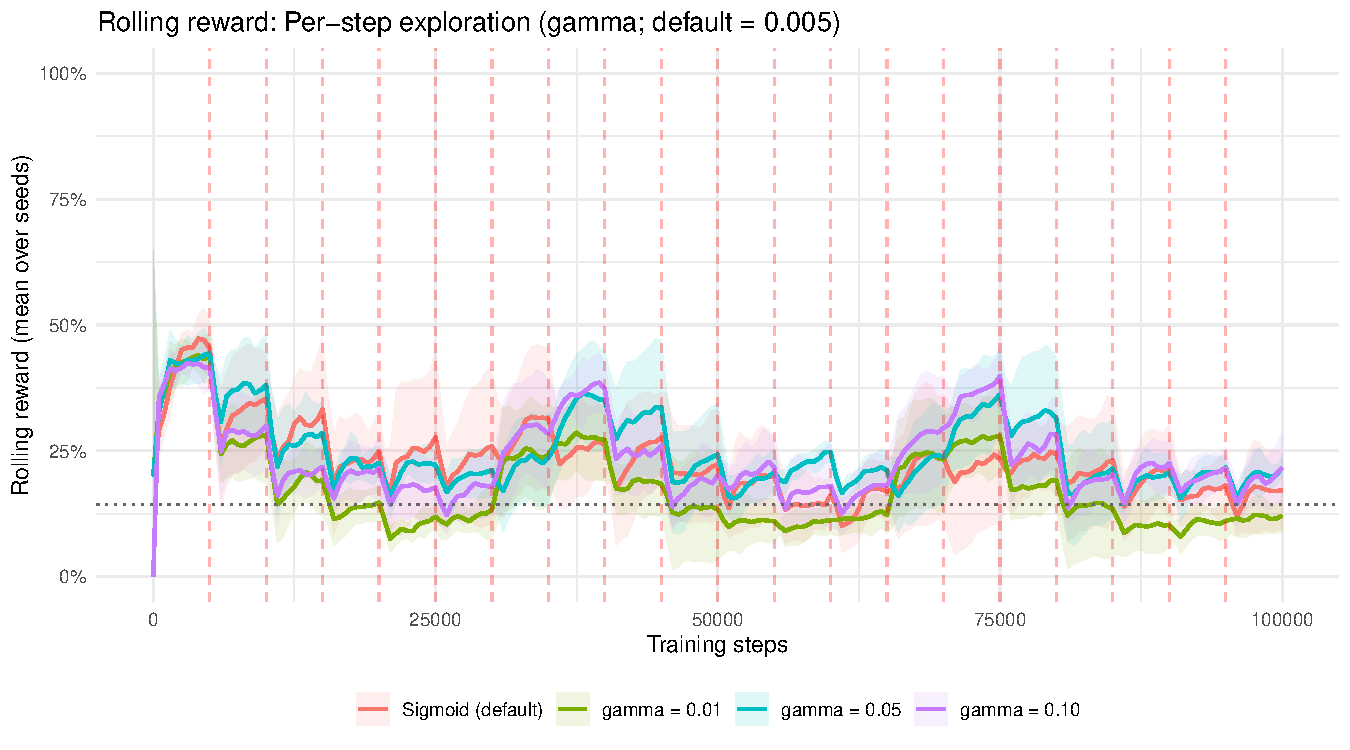
\includegraphics[keepaspectratio]{NeuralBandit_Metric_Mapping_files/figure-pdf/curves-2.pdf}}

\pandocbounded{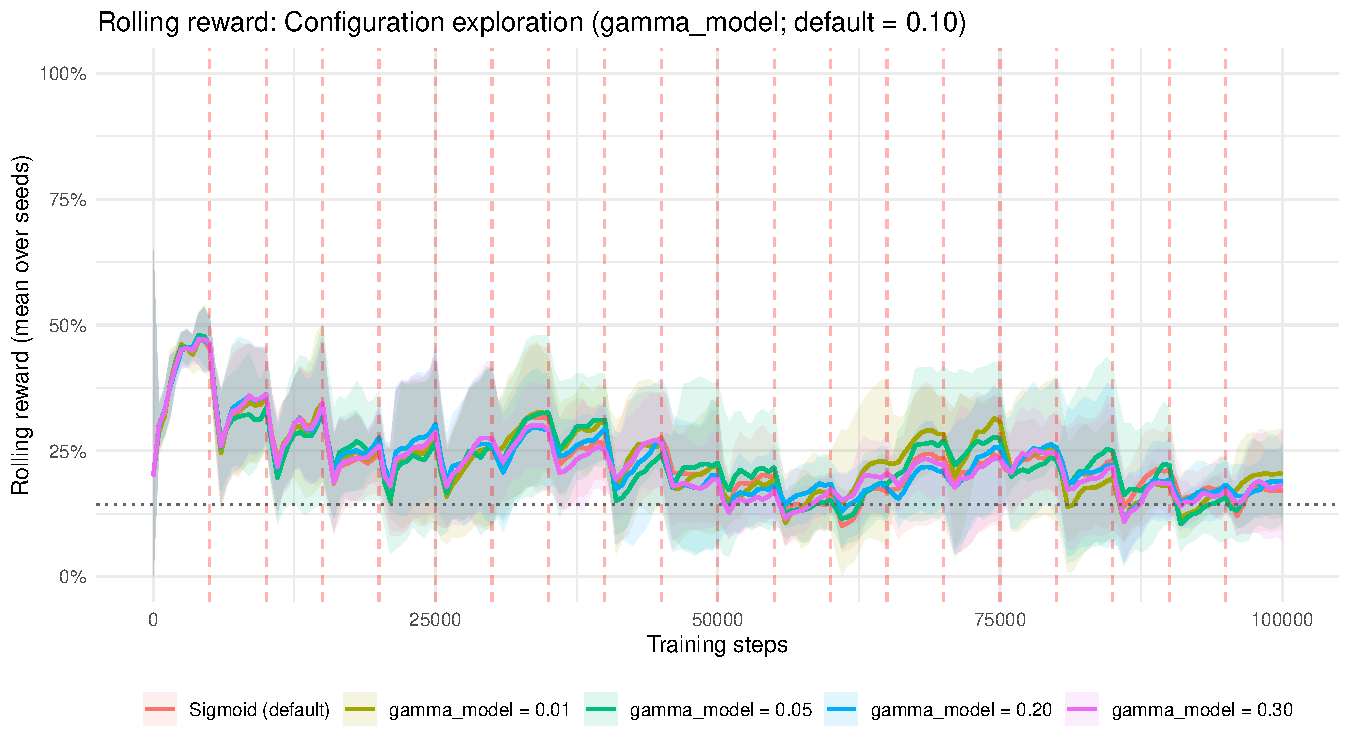
\includegraphics[keepaspectratio]{NeuralBandit_Metric_Mapping_files/figure-pdf/curves-3.pdf}}

\pandocbounded{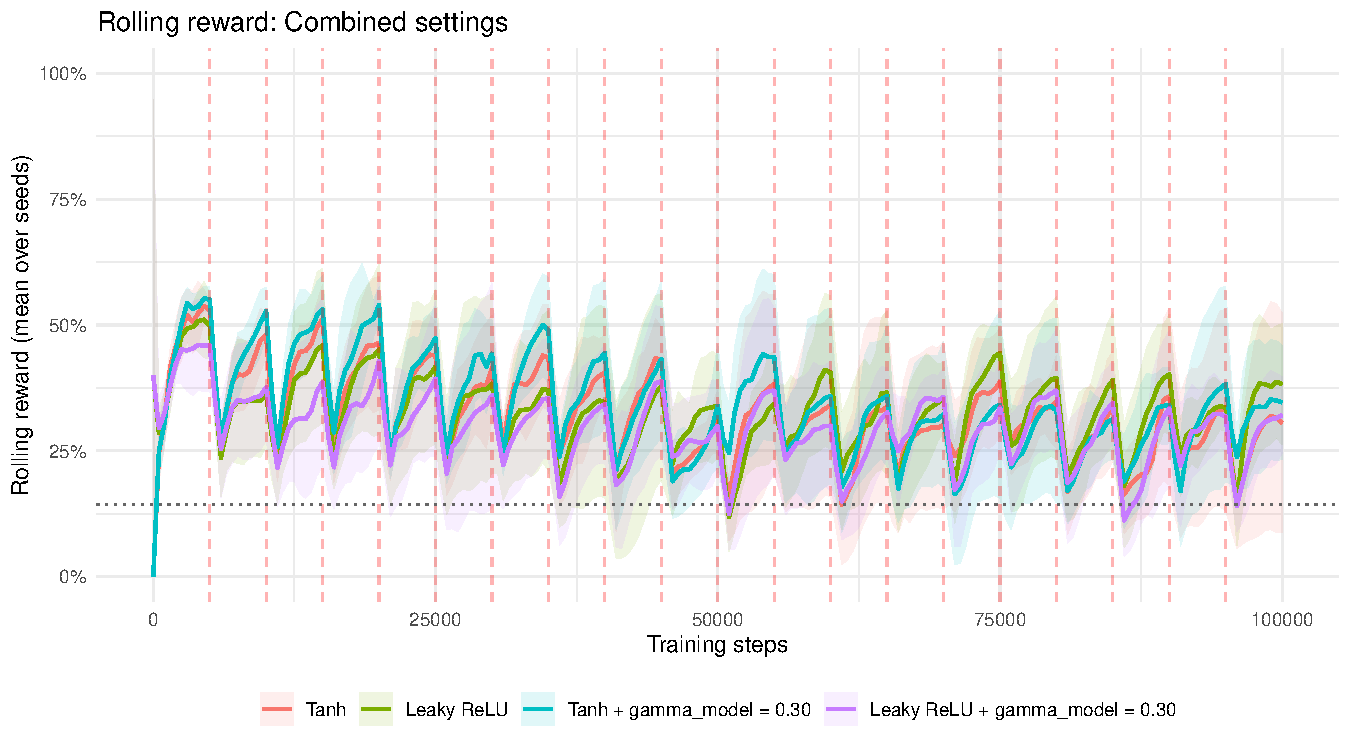
\includegraphics[keepaspectratio]{NeuralBandit_Metric_Mapping_files/figure-pdf/curves-4.pdf}}

\section{Recovery map}\label{recovery-map}

Share of seeds in which each drift was recovered (1 = every seed).

\pandocbounded{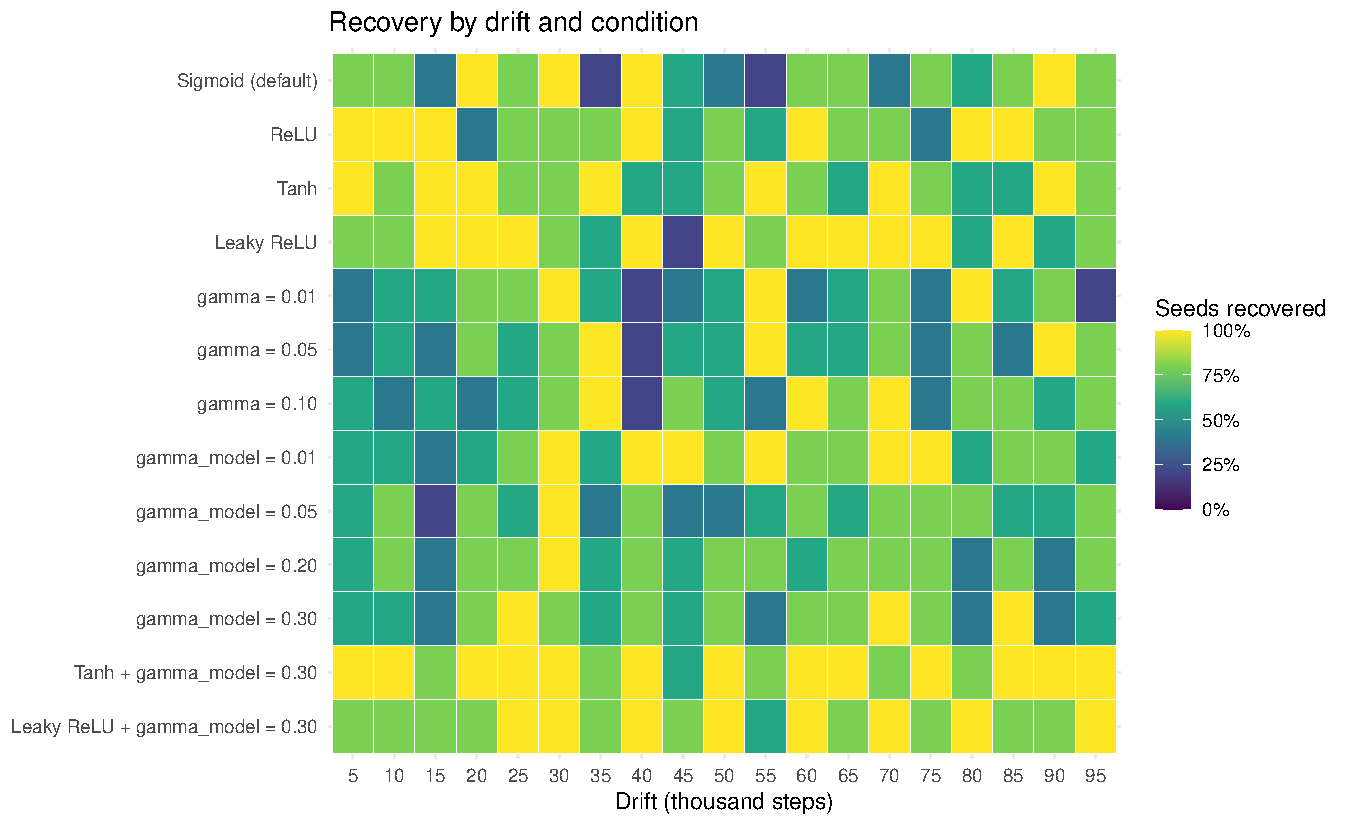
\includegraphics[keepaspectratio]{NeuralBandit_Metric_Mapping_files/figure-pdf/recovery-map-1.pdf}}

\section{Appendix: individual runs (first seed of each
condition)}\label{appendix-individual-runs-first-seed-of-each-condition}

\pandocbounded{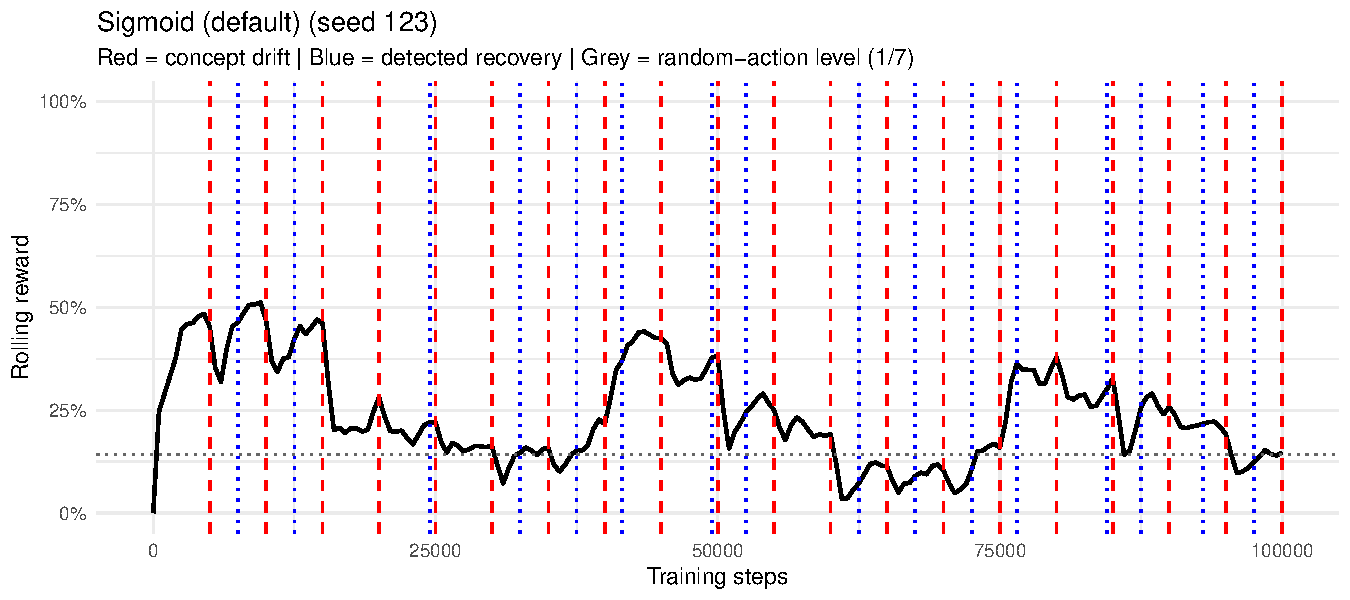
\includegraphics[keepaspectratio]{NeuralBandit_Metric_Mapping_files/figure-pdf/single-runs-1.pdf}}

\begin{verbatim}


| drift_step|recovered | recovery_step| recovery_time| rolling_reward|
|----------:|:---------|-------------:|-------------:|--------------:|
|       5000|TRUE      |          7500|          2500|          0.463|
|      10000|TRUE      |         12500|          2500|          0.423|
|      15000|FALSE     |            NA|            NA|             NA|
|      20000|TRUE      |         24500|          4500|          0.220|
|      25000|FALSE     |            NA|            NA|             NA|
|      30000|TRUE      |         32500|          2500|          0.147|
|      35000|TRUE      |         37500|          2500|          0.153|
|      40000|TRUE      |         41500|          1500|          0.369|
|      45000|TRUE      |         49500|          4500|          0.378|
|      50000|TRUE      |         52500|          2500|          0.244|
|      55000|FALSE     |            NA|            NA|             NA|
|      60000|TRUE      |         62500|          2500|          0.072|
|      65000|TRUE      |         67500|          2500|          0.090|
|      70000|TRUE      |         72500|          2500|          0.106|
|      75000|TRUE      |         76500|          1500|          0.363|
|      80000|TRUE      |         84500|          4500|          0.302|
|      85000|TRUE      |         87500|          2500|          0.257|
|      90000|TRUE      |         93000|          3000|          0.217|
|      95000|TRUE      |         97500|          2500|          0.124|
\end{verbatim}

\pandocbounded{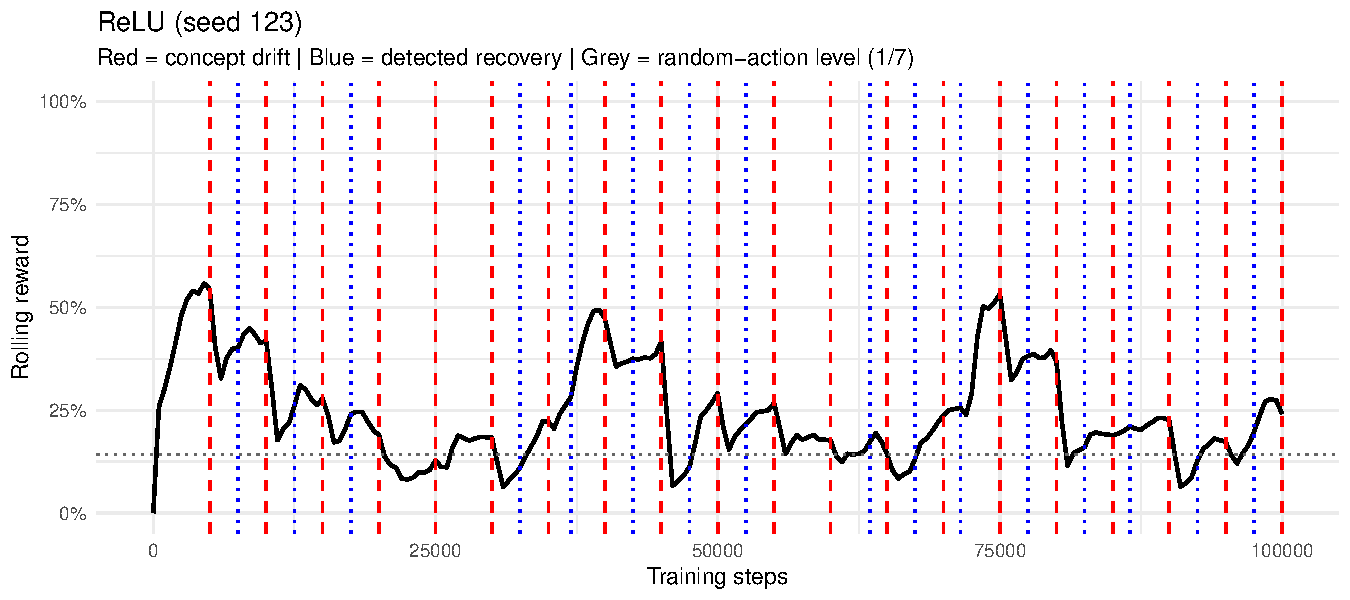
\includegraphics[keepaspectratio]{NeuralBandit_Metric_Mapping_files/figure-pdf/single-runs-2.pdf}}

\begin{verbatim}


| drift_step|recovered | recovery_step| recovery_time| rolling_reward|
|----------:|:---------|-------------:|-------------:|--------------:|
|       5000|TRUE      |          7500|          2500|          0.401|
|      10000|TRUE      |         12500|          2500|          0.260|
|      15000|TRUE      |         17500|          2500|          0.240|
|      20000|FALSE     |            NA|            NA|             NA|
|      25000|FALSE     |            NA|            NA|             NA|
|      30000|TRUE      |         32500|          2500|          0.110|
|      35000|TRUE      |         37000|          2000|          0.282|
|      40000|TRUE      |         42500|          2500|          0.375|
|      45000|TRUE      |         47500|          2500|          0.112|
|      50000|TRUE      |         52500|          2500|          0.216|
|      55000|FALSE     |            NA|            NA|             NA|
|      60000|TRUE      |         63500|          3500|          0.174|
|      65000|TRUE      |         67500|          2500|          0.133|
|      70000|TRUE      |         71500|          1500|          0.256|
|      75000|TRUE      |         77500|          2500|          0.382|
|      80000|TRUE      |         82500|          2500|          0.160|
|      85000|TRUE      |         86500|          1500|          0.210|
|      90000|TRUE      |         92500|          2500|          0.128|
|      95000|TRUE      |         97500|          2500|          0.196|
\end{verbatim}

\pandocbounded{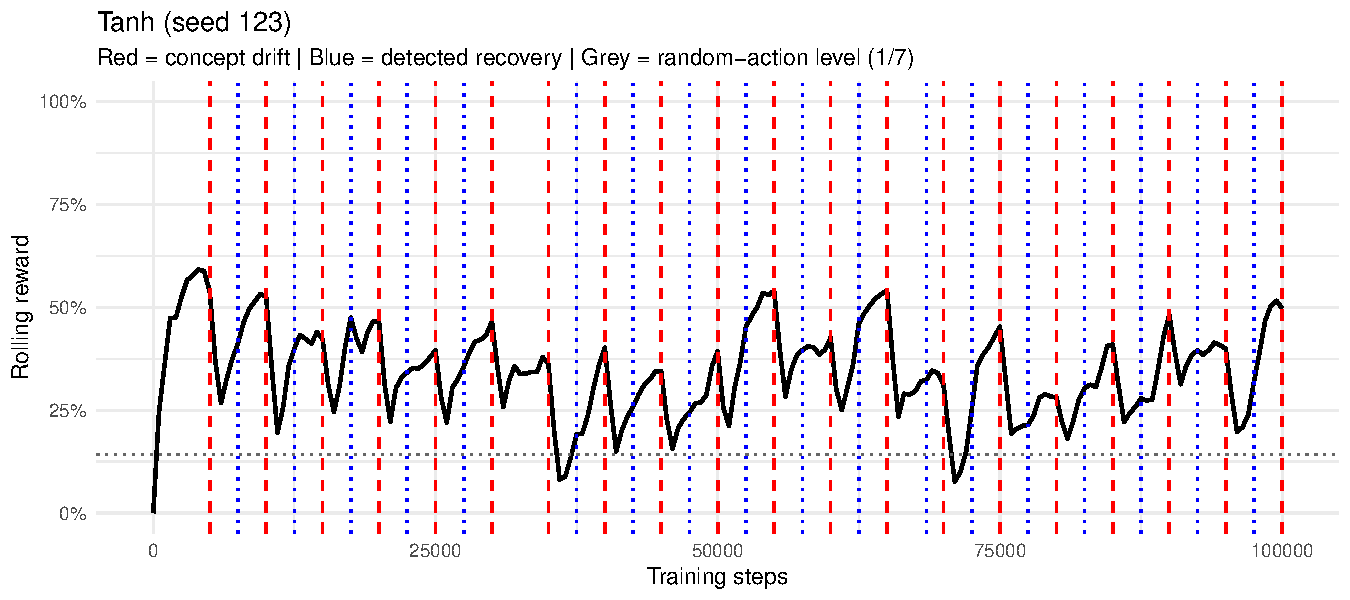
\includegraphics[keepaspectratio]{NeuralBandit_Metric_Mapping_files/figure-pdf/single-runs-3.pdf}}

\begin{verbatim}


| drift_step|recovered | recovery_step| recovery_time| rolling_reward|
|----------:|:---------|-------------:|-------------:|--------------:|
|       5000|TRUE      |          7500|          2500|          0.412|
|      10000|TRUE      |         12500|          2500|          0.400|
|      15000|TRUE      |         17500|          2500|          0.475|
|      20000|TRUE      |         22500|          2500|          0.342|
|      25000|TRUE      |         27500|          2500|          0.355|
|      30000|FALSE     |            NA|            NA|             NA|
|      35000|TRUE      |         37500|          2500|          0.191|
|      40000|TRUE      |         42500|          2500|          0.258|
|      45000|TRUE      |         47500|          2500|          0.244|
|      50000|TRUE      |         52500|          2500|          0.452|
|      55000|TRUE      |         57500|          2500|          0.396|
|      60000|TRUE      |         62500|          2500|          0.461|
|      65000|TRUE      |         68500|          3500|          0.324|
|      70000|TRUE      |         72500|          2500|          0.251|
|      75000|TRUE      |         77500|          2500|          0.214|
|      80000|TRUE      |         82500|          2500|          0.303|
|      85000|TRUE      |         87500|          2500|          0.279|
|      90000|TRUE      |         92500|          2500|          0.395|
|      95000|TRUE      |         97500|          2500|          0.319|
\end{verbatim}

\pandocbounded{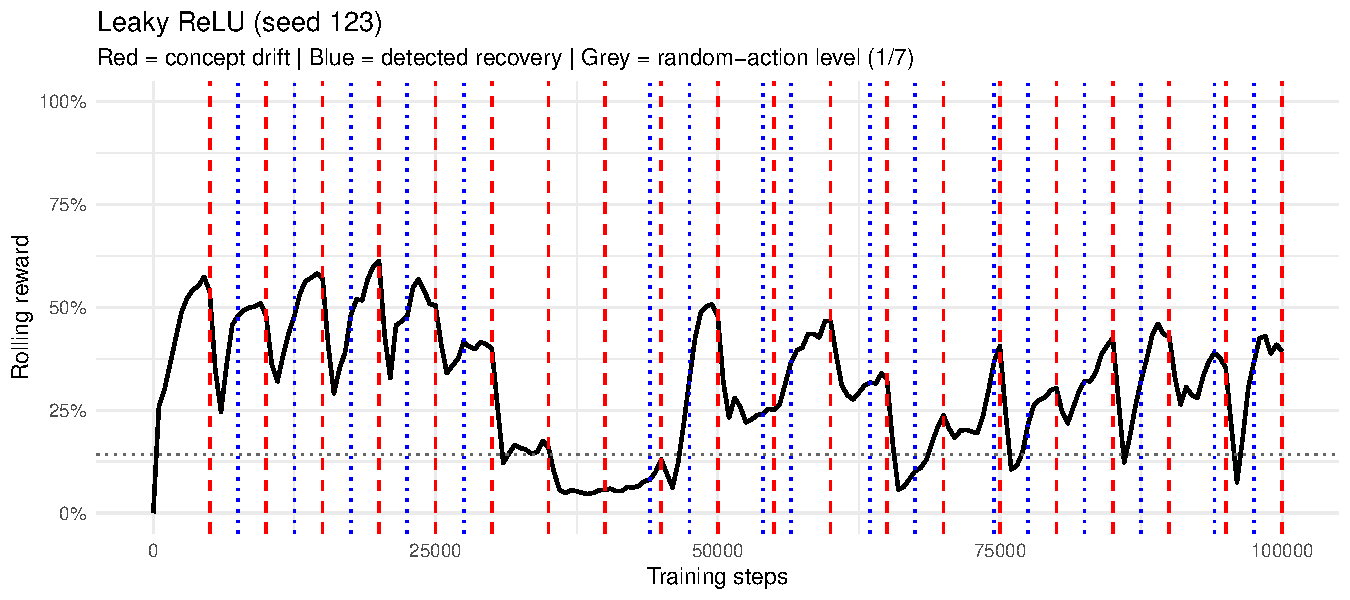
\includegraphics[keepaspectratio]{NeuralBandit_Metric_Mapping_files/figure-pdf/single-runs-4.pdf}}

\begin{verbatim}


| drift_step|recovered | recovery_step| recovery_time| rolling_reward|
|----------:|:---------|-------------:|-------------:|--------------:|
|       5000|TRUE      |          7500|          2500|          0.480|
|      10000|TRUE      |         12500|          2500|          0.479|
|      15000|TRUE      |         17500|          2500|          0.481|
|      20000|TRUE      |         22500|          2500|          0.478|
|      25000|TRUE      |         27500|          2500|          0.417|
|      30000|FALSE     |            NA|            NA|             NA|
|      35000|FALSE     |            NA|            NA|             NA|
|      40000|TRUE      |         44000|          4000|          0.081|
|      45000|TRUE      |         47500|          2500|          0.326|
|      50000|TRUE      |         54000|          4000|          0.241|
|      55000|TRUE      |         56500|          1500|          0.367|
|      60000|TRUE      |         63500|          3500|          0.317|
|      65000|TRUE      |         67500|          2500|          0.102|
|      70000|TRUE      |         74500|          4500|          0.369|
|      75000|TRUE      |         77500|          2500|          0.216|
|      80000|TRUE      |         82500|          2500|          0.321|
|      85000|TRUE      |         87500|          2500|          0.321|
|      90000|TRUE      |         94000|          4000|          0.389|
|      95000|TRUE      |         97500|          2500|          0.366|
\end{verbatim}

\pandocbounded{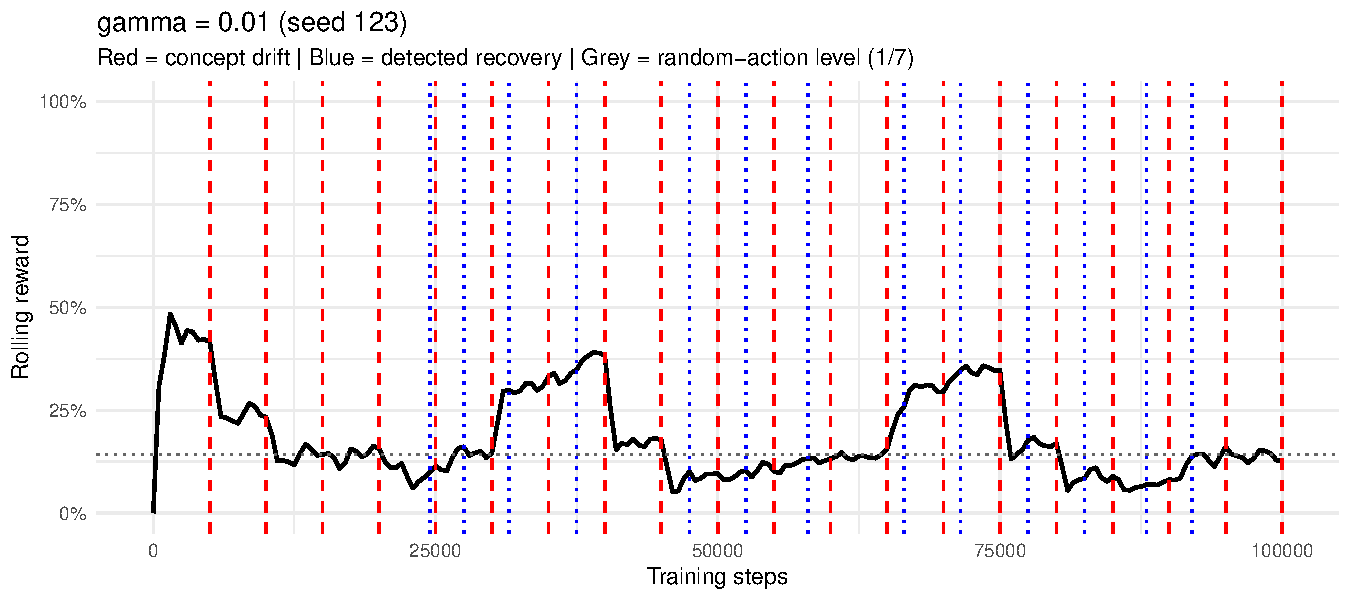
\includegraphics[keepaspectratio]{NeuralBandit_Metric_Mapping_files/figure-pdf/single-runs-5.pdf}}

\begin{verbatim}


| drift_step|recovered | recovery_step| recovery_time| rolling_reward|
|----------:|:---------|-------------:|-------------:|--------------:|
|       5000|FALSE     |            NA|            NA|             NA|
|      10000|FALSE     |            NA|            NA|             NA|
|      15000|FALSE     |            NA|            NA|             NA|
|      20000|TRUE      |         24500|          4500|          0.098|
|      25000|TRUE      |         27500|          2500|          0.161|
|      30000|TRUE      |         31500|          1500|          0.299|
|      35000|TRUE      |         37500|          2500|          0.348|
|      40000|FALSE     |            NA|            NA|             NA|
|      45000|TRUE      |         47500|          2500|          0.100|
|      50000|TRUE      |         52500|          2500|          0.103|
|      55000|TRUE      |         58000|          3000|          0.132|
|      60000|FALSE     |            NA|            NA|             NA|
|      65000|TRUE      |         66500|          1500|          0.257|
|      70000|TRUE      |         71500|          1500|          0.347|
|      75000|TRUE      |         77500|          2500|          0.177|
|      80000|TRUE      |         82500|          2500|          0.084|
|      85000|TRUE      |         88000|          3000|          0.069|
|      90000|TRUE      |         92000|          2000|          0.138|
|      95000|FALSE     |            NA|            NA|             NA|
\end{verbatim}

\pandocbounded{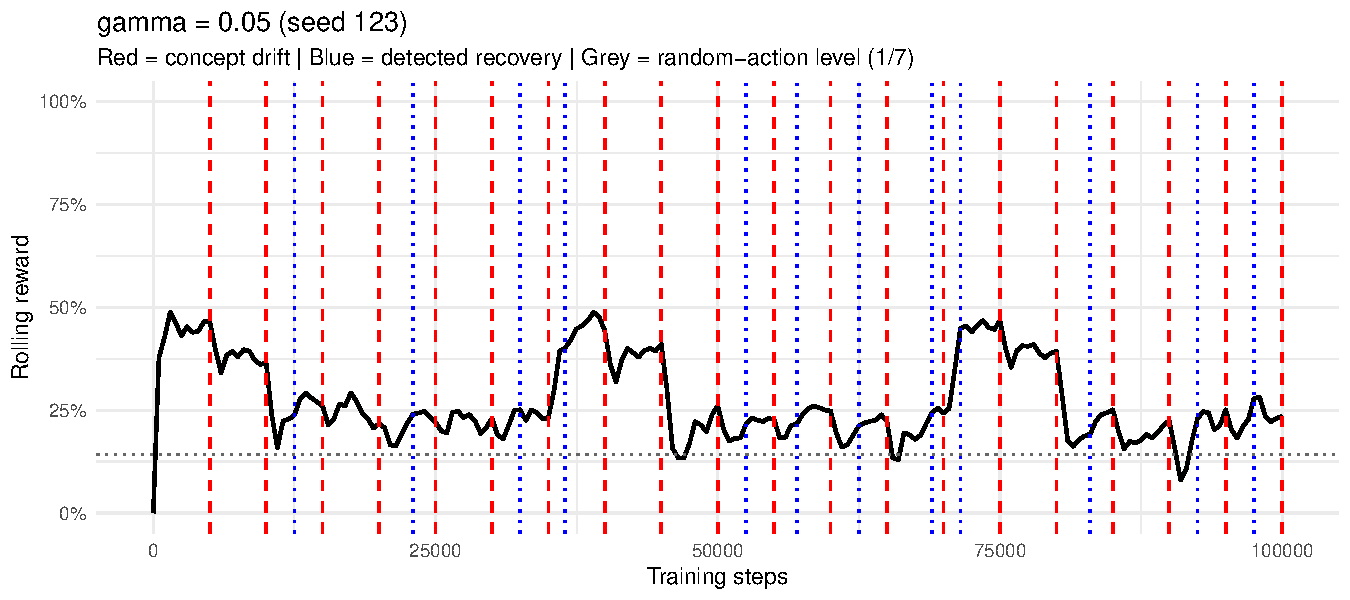
\includegraphics[keepaspectratio]{NeuralBandit_Metric_Mapping_files/figure-pdf/single-runs-6.pdf}}

\begin{verbatim}


| drift_step|recovered | recovery_step| recovery_time| rolling_reward|
|----------:|:---------|-------------:|-------------:|--------------:|
|       5000|FALSE     |            NA|            NA|             NA|
|      10000|TRUE      |         12500|          2500|          0.238|
|      15000|FALSE     |            NA|            NA|             NA|
|      20000|TRUE      |         23000|          3000|          0.240|
|      25000|FALSE     |            NA|            NA|             NA|
|      30000|TRUE      |         32500|          2500|          0.251|
|      35000|TRUE      |         36500|          1500|          0.402|
|      40000|FALSE     |            NA|            NA|             NA|
|      45000|FALSE     |            NA|            NA|             NA|
|      50000|TRUE      |         52500|          2500|          0.215|
|      55000|TRUE      |         57000|          2000|          0.216|
|      60000|TRUE      |         62500|          2500|          0.212|
|      65000|TRUE      |         69000|          4000|          0.244|
|      70000|TRUE      |         71500|          1500|          0.449|
|      75000|FALSE     |            NA|            NA|             NA|
|      80000|TRUE      |         83000|          3000|          0.192|
|      85000|FALSE     |            NA|            NA|             NA|
|      90000|TRUE      |         92500|          2500|          0.229|
|      95000|TRUE      |         97500|          2500|          0.278|
\end{verbatim}

\pandocbounded{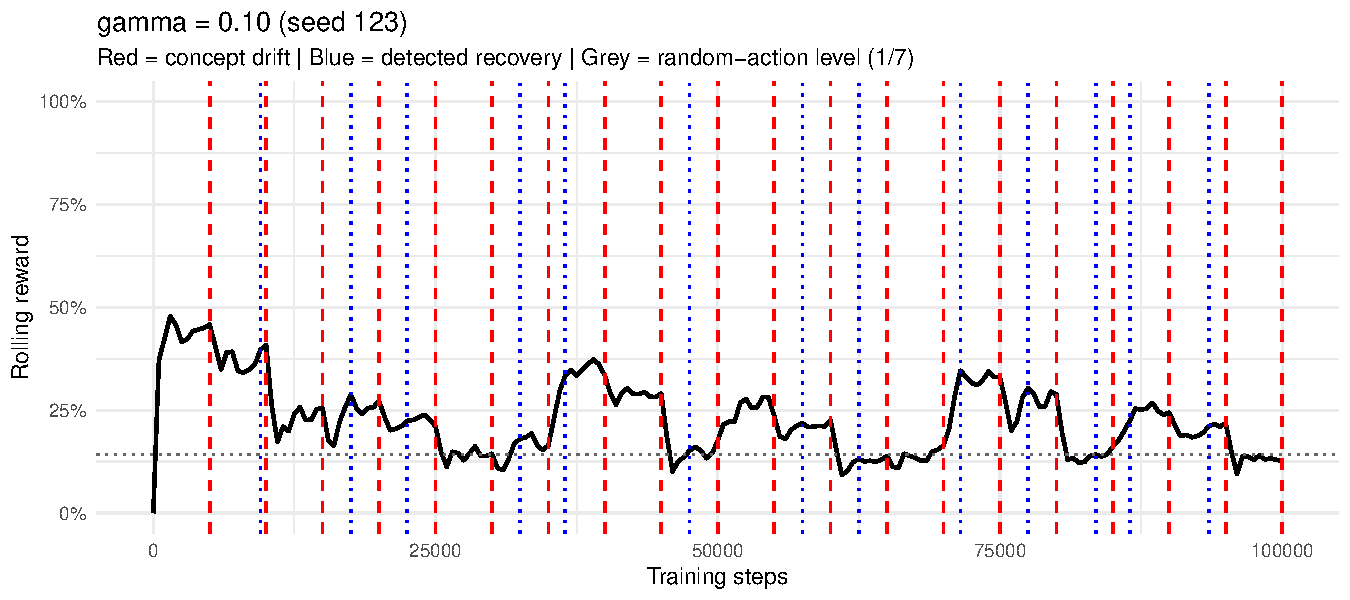
\includegraphics[keepaspectratio]{NeuralBandit_Metric_Mapping_files/figure-pdf/single-runs-7.pdf}}

\begin{verbatim}


| drift_step|recovered | recovery_step| recovery_time| rolling_reward|
|----------:|:---------|-------------:|-------------:|--------------:|
|       5000|TRUE      |          9500|          4500|          0.397|
|      10000|FALSE     |            NA|            NA|             NA|
|      15000|TRUE      |         17500|          2500|          0.288|
|      20000|TRUE      |         22500|          2500|          0.224|
|      25000|FALSE     |            NA|            NA|             NA|
|      30000|TRUE      |         32500|          2500|          0.180|
|      35000|TRUE      |         36500|          1500|          0.335|
|      40000|FALSE     |            NA|            NA|             NA|
|      45000|TRUE      |         47500|          2500|          0.151|
|      50000|FALSE     |            NA|            NA|             NA|
|      55000|TRUE      |         57500|          2500|          0.218|
|      60000|TRUE      |         62500|          2500|          0.131|
|      65000|FALSE     |            NA|            NA|             NA|
|      70000|TRUE      |         71500|          1500|          0.346|
|      75000|TRUE      |         77500|          2500|          0.304|
|      80000|TRUE      |         83500|          3500|          0.142|
|      85000|TRUE      |         86500|          1500|          0.224|
|      90000|TRUE      |         93500|          3500|          0.211|
|      95000|FALSE     |            NA|            NA|             NA|
\end{verbatim}

\pandocbounded{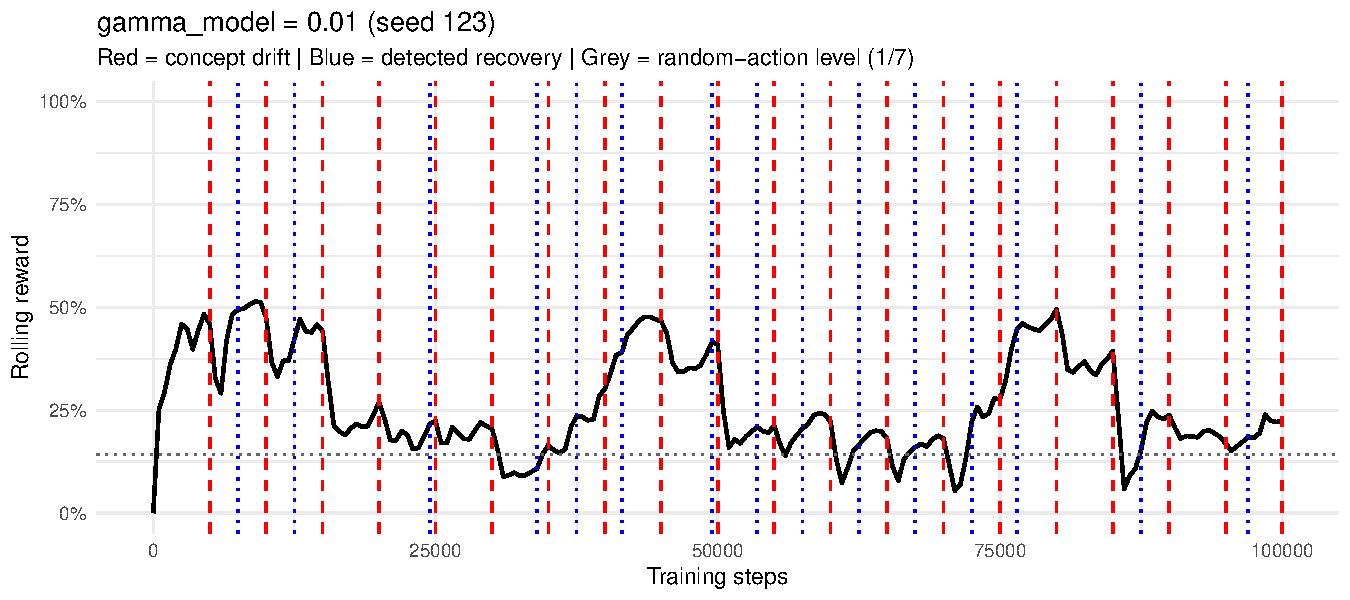
\includegraphics[keepaspectratio]{NeuralBandit_Metric_Mapping_files/figure-pdf/single-runs-8.pdf}}

\begin{verbatim}


| drift_step|recovered | recovery_step| recovery_time| rolling_reward|
|----------:|:---------|-------------:|-------------:|--------------:|
|       5000|TRUE      |          7500|          2500|          0.494|
|      10000|TRUE      |         12500|          2500|          0.423|
|      15000|FALSE     |            NA|            NA|             NA|
|      20000|TRUE      |         24500|          4500|          0.216|
|      25000|FALSE     |            NA|            NA|             NA|
|      30000|TRUE      |         34000|          4000|          0.108|
|      35000|TRUE      |         37500|          2500|          0.236|
|      40000|TRUE      |         41500|          1500|          0.390|
|      45000|TRUE      |         49500|          4500|          0.416|
|      50000|TRUE      |         53500|          3500|          0.209|
|      55000|TRUE      |         57500|          2500|          0.205|
|      60000|TRUE      |         62500|          2500|          0.165|
|      65000|TRUE      |         67500|          2500|          0.160|
|      70000|TRUE      |         72500|          2500|          0.221|
|      75000|TRUE      |         76500|          1500|          0.446|
|      80000|FALSE     |            NA|            NA|             NA|
|      85000|TRUE      |         87500|          2500|          0.153|
|      90000|FALSE     |            NA|            NA|             NA|
|      95000|TRUE      |         97000|          2000|          0.184|
\end{verbatim}

\pandocbounded{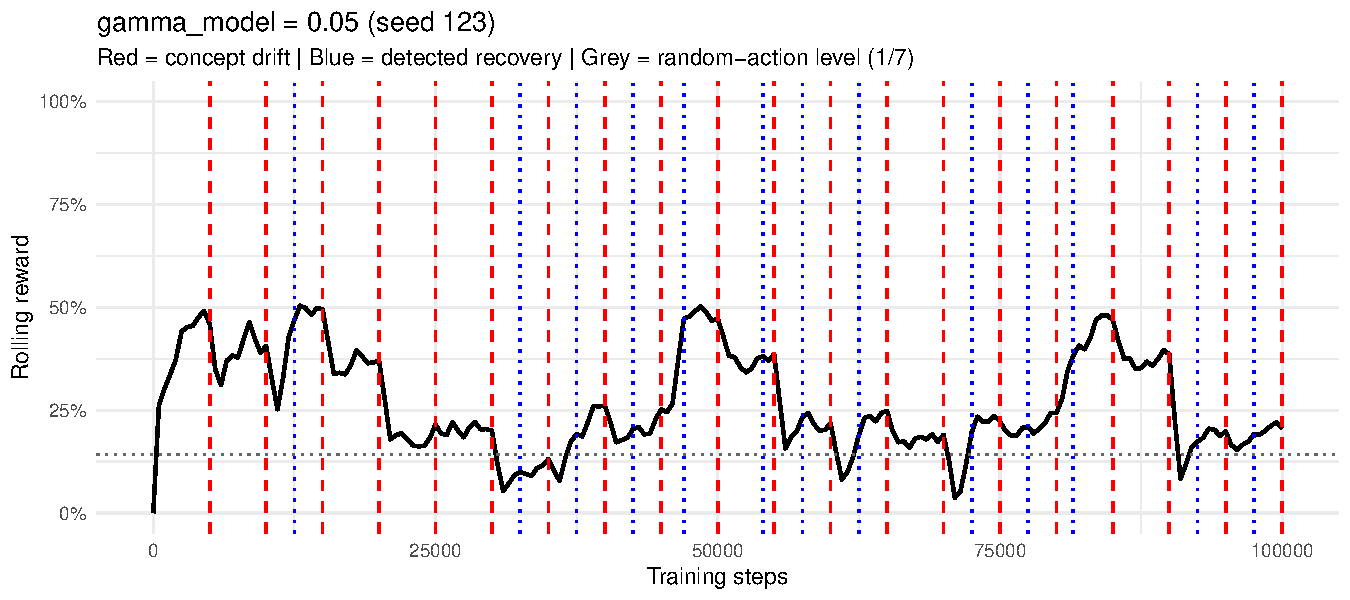
\includegraphics[keepaspectratio]{NeuralBandit_Metric_Mapping_files/figure-pdf/single-runs-9.pdf}}

\begin{verbatim}


| drift_step|recovered | recovery_step| recovery_time| rolling_reward|
|----------:|:---------|-------------:|-------------:|--------------:|
|       5000|FALSE     |            NA|            NA|             NA|
|      10000|TRUE      |         12500|          2500|          0.469|
|      15000|FALSE     |            NA|            NA|             NA|
|      20000|FALSE     |            NA|            NA|             NA|
|      25000|FALSE     |            NA|            NA|             NA|
|      30000|TRUE      |         32500|          2500|          0.099|
|      35000|TRUE      |         37500|          2500|          0.192|
|      40000|TRUE      |         42500|          2500|          0.204|
|      45000|TRUE      |         47000|          2000|          0.472|
|      50000|TRUE      |         54000|          4000|          0.381|
|      55000|TRUE      |         57500|          2500|          0.233|
|      60000|TRUE      |         62500|          2500|          0.189|
|      65000|FALSE     |            NA|            NA|             NA|
|      70000|TRUE      |         72500|          2500|          0.196|
|      75000|TRUE      |         77500|          2500|          0.209|
|      80000|TRUE      |         81500|          1500|          0.383|
|      85000|FALSE     |            NA|            NA|             NA|
|      90000|TRUE      |         92500|          2500|          0.173|
|      95000|TRUE      |         97500|          2500|          0.192|
\end{verbatim}

\pandocbounded{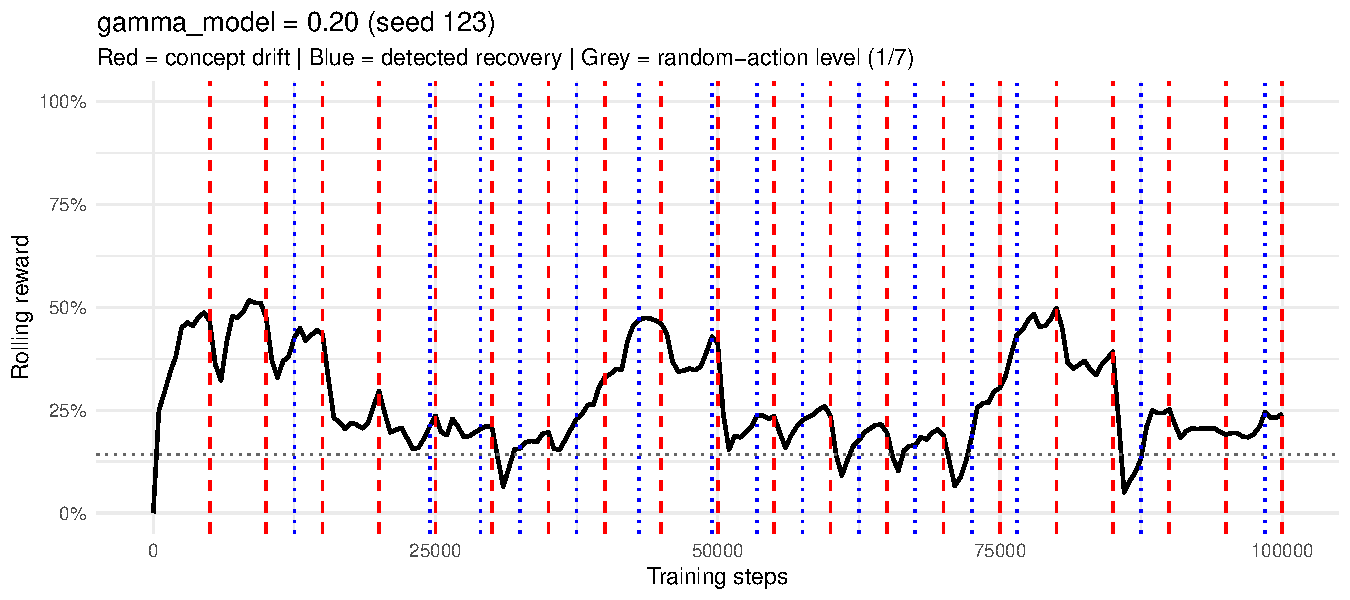
\includegraphics[keepaspectratio]{NeuralBandit_Metric_Mapping_files/figure-pdf/single-runs-10.pdf}}

\begin{verbatim}


| drift_step|recovered | recovery_step| recovery_time| rolling_reward|
|----------:|:---------|-------------:|-------------:|--------------:|
|       5000|FALSE     |            NA|            NA|             NA|
|      10000|TRUE      |         12500|          2500|          0.426|
|      15000|FALSE     |            NA|            NA|             NA|
|      20000|TRUE      |         24500|          4500|          0.211|
|      25000|TRUE      |         29000|          4000|          0.204|
|      30000|TRUE      |         32500|          2500|          0.157|
|      35000|TRUE      |         37500|          2500|          0.229|
|      40000|TRUE      |         43000|          3000|          0.469|
|      45000|TRUE      |         49500|          4500|          0.429|
|      50000|TRUE      |         53500|          3500|          0.238|
|      55000|TRUE      |         57500|          2500|          0.225|
|      60000|TRUE      |         62500|          2500|          0.176|
|      65000|TRUE      |         67500|          2500|          0.164|
|      70000|TRUE      |         72500|          2500|          0.185|
|      75000|TRUE      |         76500|          1500|          0.433|
|      80000|FALSE     |            NA|            NA|             NA|
|      85000|TRUE      |         87500|          2500|          0.133|
|      90000|FALSE     |            NA|            NA|             NA|
|      95000|TRUE      |         98500|          3500|          0.246|
\end{verbatim}

\pandocbounded{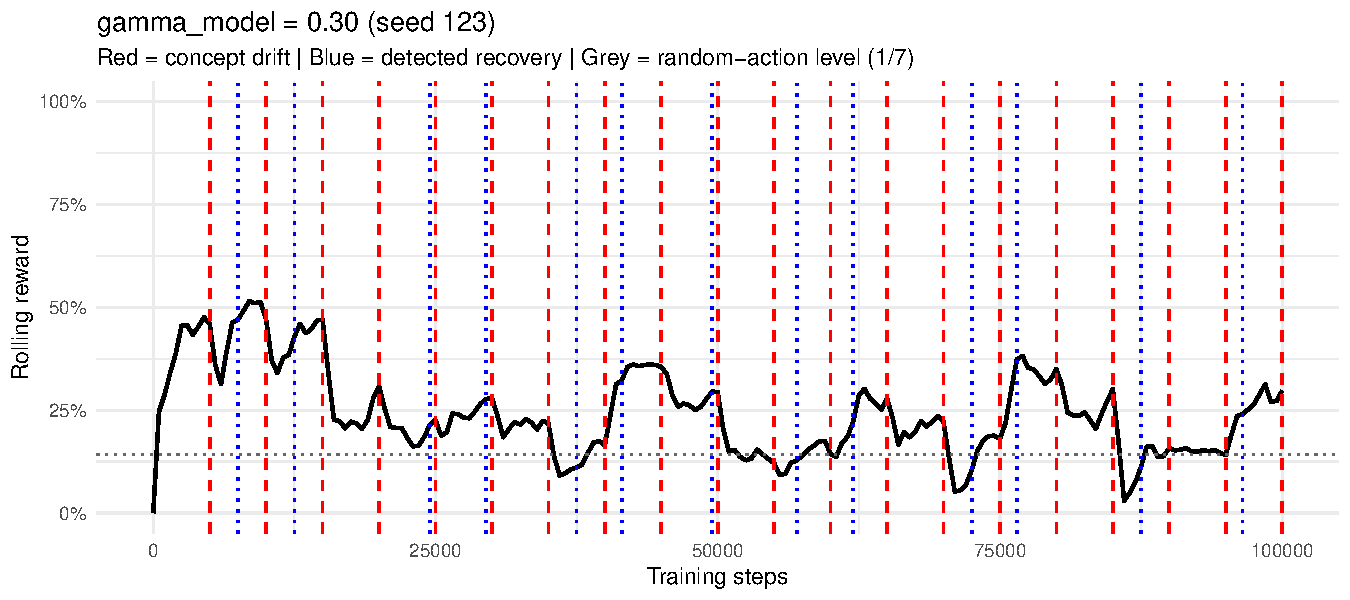
\includegraphics[keepaspectratio]{NeuralBandit_Metric_Mapping_files/figure-pdf/single-runs-11.pdf}}

\begin{verbatim}


| drift_step|recovered | recovery_step| recovery_time| rolling_reward|
|----------:|:---------|-------------:|-------------:|--------------:|
|       5000|TRUE      |          7500|          2500|          0.470|
|      10000|TRUE      |         12500|          2500|          0.429|
|      15000|FALSE     |            NA|            NA|             NA|
|      20000|TRUE      |         24500|          4500|          0.214|
|      25000|TRUE      |         29500|          4500|          0.277|
|      30000|FALSE     |            NA|            NA|             NA|
|      35000|TRUE      |         37500|          2500|          0.111|
|      40000|TRUE      |         41500|          1500|          0.322|
|      45000|TRUE      |         49500|          4500|          0.295|
|      50000|FALSE     |            NA|            NA|             NA|
|      55000|TRUE      |         57000|          2000|          0.128|
|      60000|TRUE      |         62000|          2000|          0.222|
|      65000|FALSE     |            NA|            NA|             NA|
|      70000|TRUE      |         72500|          2500|          0.104|
|      75000|TRUE      |         76500|          1500|          0.373|
|      80000|FALSE     |            NA|            NA|             NA|
|      85000|TRUE      |         87500|          2500|          0.112|
|      90000|FALSE     |            NA|            NA|             NA|
|      95000|TRUE      |         96500|          1500|          0.241|
\end{verbatim}

\pandocbounded{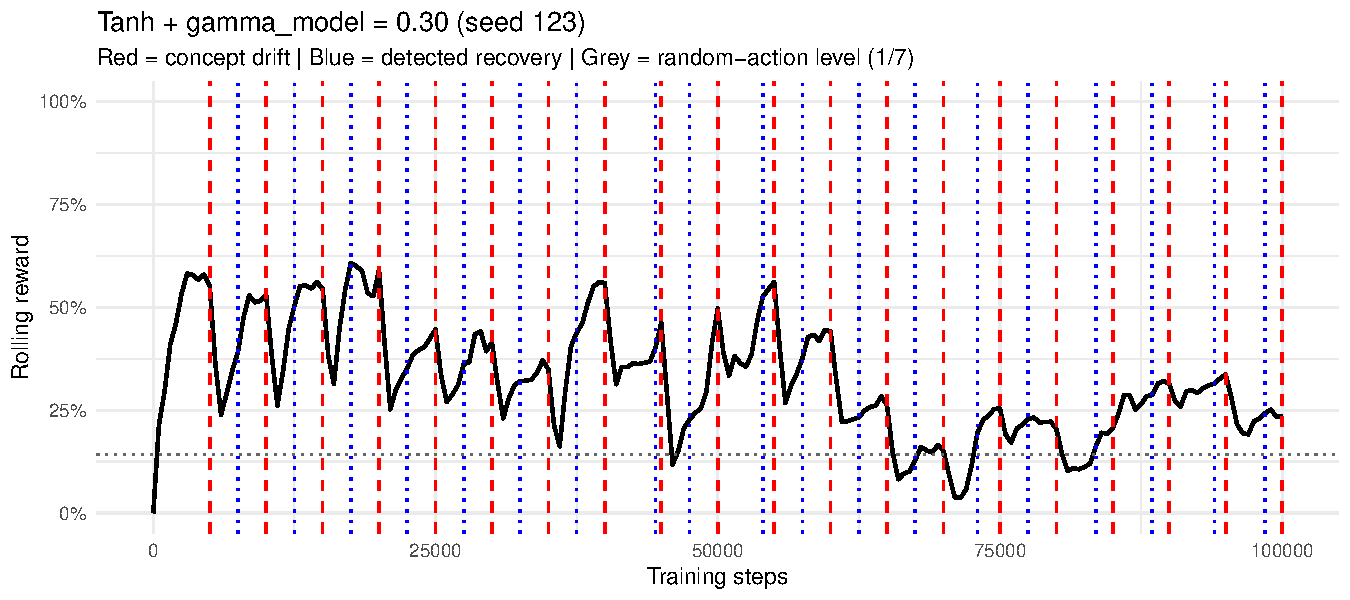
\includegraphics[keepaspectratio]{NeuralBandit_Metric_Mapping_files/figure-pdf/single-runs-12.pdf}}

\begin{verbatim}


| drift_step|recovered | recovery_step| recovery_time| rolling_reward|
|----------:|:---------|-------------:|-------------:|--------------:|
|       5000|TRUE      |          7500|          2500|          0.391|
|      10000|TRUE      |         12500|          2500|          0.503|
|      15000|TRUE      |         17500|          2500|          0.608|
|      20000|TRUE      |         22500|          2500|          0.353|
|      25000|TRUE      |         27500|          2500|          0.362|
|      30000|TRUE      |         32500|          2500|          0.320|
|      35000|TRUE      |         37500|          2500|          0.438|
|      40000|TRUE      |         44500|          4500|          0.403|
|      45000|TRUE      |         47500|          2500|          0.227|
|      50000|TRUE      |         54000|          4000|          0.526|
|      55000|TRUE      |         57500|          2500|          0.375|
|      60000|TRUE      |         62500|          2500|          0.232|
|      65000|TRUE      |         67500|          2500|          0.128|
|      70000|TRUE      |         73000|          3000|          0.194|
|      75000|TRUE      |         77500|          2500|          0.228|
|      80000|TRUE      |         83500|          3500|          0.162|
|      85000|TRUE      |         88500|          3500|          0.287|
|      90000|TRUE      |         94000|          4000|          0.315|
|      95000|TRUE      |         98500|          3500|          0.243|
\end{verbatim}

\pandocbounded{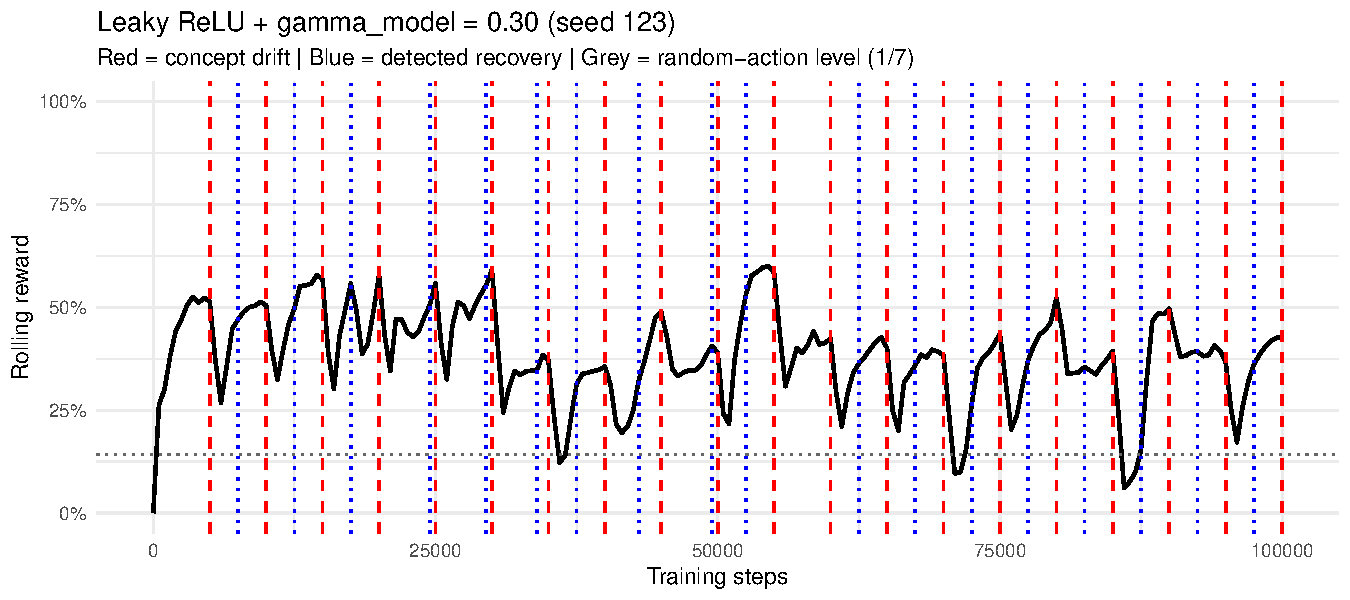
\includegraphics[keepaspectratio]{NeuralBandit_Metric_Mapping_files/figure-pdf/single-runs-13.pdf}}

\begin{verbatim}


| drift_step|recovered | recovery_step| recovery_time| rolling_reward|
|----------:|:---------|-------------:|-------------:|--------------:|
|       5000|TRUE      |          7500|          2500|          0.470|
|      10000|TRUE      |         12500|          2500|          0.497|
|      15000|TRUE      |         17500|          2500|          0.558|
|      20000|TRUE      |         24500|          4500|          0.506|
|      25000|TRUE      |         29500|          4500|          0.555|
|      30000|TRUE      |         34000|          4000|          0.348|
|      35000|TRUE      |         37500|          2500|          0.313|
|      40000|TRUE      |         43000|          3000|          0.322|
|      45000|TRUE      |         49500|          4500|          0.406|
|      50000|TRUE      |         52500|          2500|          0.531|
|      55000|FALSE     |            NA|            NA|             NA|
|      60000|TRUE      |         62500|          2500|          0.363|
|      65000|TRUE      |         67500|          2500|          0.359|
|      70000|TRUE      |         72500|          2500|          0.264|
|      75000|TRUE      |         77500|          2500|          0.371|
|      80000|TRUE      |         82500|          2500|          0.355|
|      85000|TRUE      |         87500|          2500|          0.154|
|      90000|TRUE      |         92500|          2500|          0.393|
|      95000|TRUE      |         97500|          2500|          0.362|
\end{verbatim}




\end{document}
